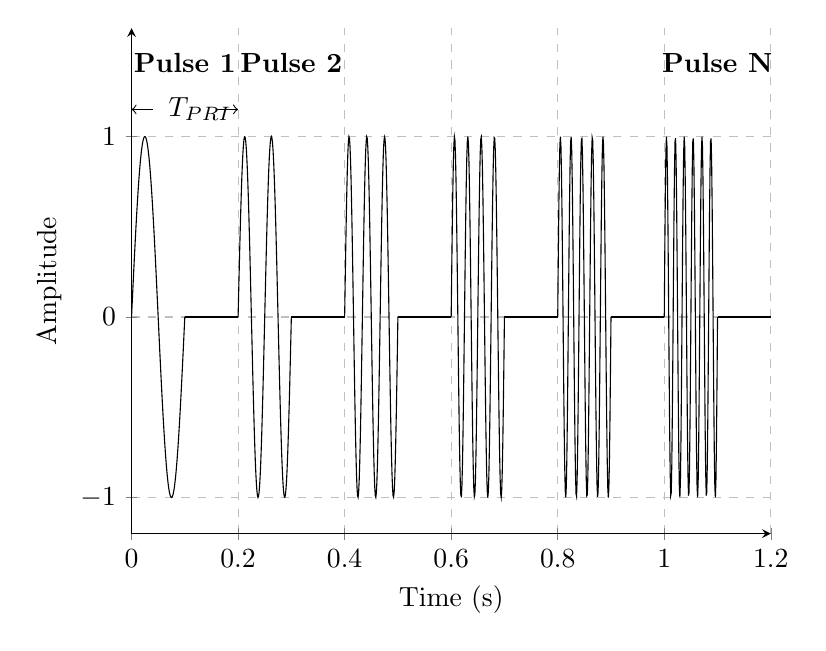
\begin{tikzpicture}
        \begin{axis}[
            width=0.8\textwidth,
            height=8cm,
            xlabel={Time (s)},
            ylabel={Amplitude},
            axis lines=left,
            grid=both,
            grid style={dashed},
            xmin=0,
            xmax=1.2,
            ymin=-1.2,
            ymax=1.6,
            xtick={0, 0.2, 0.4, 0.6, 0.8,1,1.2},
            ytick={-1, 0, 1},
            legend pos=north east,
            unbounded coords=discard,
        ]
        \addplot[black, domain=0:0.1, samples=100] {sin(deg(2*pi*1000.1*x))};
        \addplot[black, domain=0.1:0.2]{0};
        \addplot[black, domain=0.2:0.3, samples=100] {sin(deg(2*pi*2000.2*(x-0.2)))};;
        \addplot[black, domain=0.3:0.4]{0};
        \addplot[black, domain=0.4:0.5, samples=100] {sin(deg(2*pi*3000.3*(x-0.4)))};
        \addplot[black, domain=0.5:0.6]{0};
        \addplot[black, domain=0.6:0.7, samples=100] {sin(deg(2*pi*4000.4*(x-0.6)))};
        \addplot[black, domain=0.7:0.8]{0};
        \addplot[black, domain=0.8:0.9, samples=100] {sin(deg(2*pi*5000.5*(x-0.8)))};
        \addplot[black, domain=0.9:1]{0};
        \addplot[black, domain=1:1.1, samples=100] {sin(deg(2*pi*6000.6*(x-1)))};
        \addplot[black, domain=1.1:1.2]{0};

        % Label period
        \draw[<-] (axis cs: 0, 1.15) -- (axis cs: 0.04, 1.15) node[midway,right,xshift=6pt] {$T_{PRI}$};
        \draw[->] (axis cs: 0.16, 1.15) -- (axis cs: 0.2, 1.15);

        
        %Label Pulses
        \draw[draw=none] (axis cs: 0, 1.3) -- (axis cs: 0.2, 1.3) node[midway,above] {\textbf{Pulse 1}};
        \draw[draw=none] (axis cs: 0.2, 1.3) -- (axis cs: 0.4, 1.3) node[midway,above] {\textbf{Pulse 2}};
        \draw[draw=none] (axis cs: 1, 1.3) -- (axis cs: 1.2, 1.3) node[midway,above] {\textbf{Pulse N}};

        \end{axis}
    \end{tikzpicture}